\chapter{Background and Notation}\label{ch:background}

\section{Multi-Armed Bandits}

\subsection{The Explore-Exploit Tradeoff}
 The real-world decision-making processes has a feature that presents uncertainity 
in the outcome of future decision. 
So it is difficult for agent(decision-maker), due to uncertainity in the result of a given action, to choose the best next action. 
Most of the real-world tasks aiming at maximising cumulative outcomes require to make many sequential decisions.

Successful completion of such a task necessitates a basic tension: an decision-maker (agent) must constantly choose between exploiting all 
known good possibilities and researching unknown but potentially better options. 
This conflict is known as the explore-exploit trade-off, and it's at the basis of improving decision-making.

The explore-exploit tradeoff can be observed in a variety of natural and artificial systems. 
Foraging animals in the natural world strive to consume as much food as possible while also seeking out the most rewarding foraging areas \cite{Keasar:2002}.

\subsection{Multi-Armed Bandit Problem}
 The Multi-armed Bandit (MAB) problem is a classic mathematical description 
of the explore-exploit tradeoff \cite{Robbins:1952}. 
A decision-maker(agent) is faced with a sequential series of decisions in the MAB problem. 
Each choice requires the decision-maker(agent) to pick between two or more options, often known as arms, each of which has a probability distribution associated with it that models the reward. 
The decision-maker receives a noisy reward chosen from the related probability distribution after selecting an option. 
The goal of the decision-maker is to maximise their expected cumulative reward, 
which is comparable to selecting the option with the highest mean as often as possible.
\subsubsection{Model and Example}
We consider the basic model with \textit{IID} rewards, called \textit{stochastic bandits}\cite{mab-intro}. 
An algorithm has $K$ possible actions to choose from, a.k.a. \textit{arms}, and there are $T$ rounds, for some known $K$ and $T$ . 
In each round, the algorithm chooses an arm and collects a reward for this arm. The algorithm’s goal is to maximize its total reward over the $T$ rounds. We are primarily interested in the mean reward vector $\mu \in [0, 1]^K$, where $\mu(a) = \mathbb{E}[\mathcal{D}_a]$ is the mean reward of arm $a$.
\begin{algorithm}
%	\SetAlgoVlined
	\caption{Epsilon-greedy algorithm}
	\For{$each\ round\ t \in T$}
	{
		toss a coin with success probability $\epsilon$;\\
		\eIf{success}
		{
			explore: choose an arm uniformly at random
		}
		{
			exploit: choose the arm with the highest average reward so far
		}
	}
\end{algorithm}\\
Some motivating examples,\\
\textbf{Ad selection}: In website advertising, a user visits a webpage, and a learning algorithm selects one of many possible ads to display. If ad $a$ is displayed, the website observes whether the user clicks on the ad, in which case the advertiser pays some amount $v_a \in [0, 1]$. So each ad is an arm, and the paid amount is the reward.\\
\textbf{Medical Trials}: a patient visits a doctor and the doctor can prescribe one of several possible treatments, and observes the treatment effectiveness. Then the next patient arrives, and so forth.
\begin{definition}
	For best arm $\mu^*$ and total rounds $T$, the difference between cumulative reward to the \textit{best-arm benchmark} $\mu^* \cdot T$ is called \textit{regret} at round $T$:
	$$ R(T) = \mu^* \cdot T - \sum_{t=1}^{T}\mu(a_t) $$
\end{definition}
Since $R(T)$ is a random variable. We will typically talk about \textit{expected} regret $\mathbb{E}[R(T)]$.

\section{Bayesian Optimization}
We want to optimize a function $f : \mathcal{X} \to \mathbb{R}$ over some set $\mathcal{X}$ (here the set $\mathcal{X}$ is the set of hyperparameters we want to search over). But $f$ is expensive to compute and no access to gradients, making optimization difficult\cite{cs4787}. Main idea of Bayesian optimization:
\begin{itemize}
	\item Model $f$ as a probability distribution.
	\item If we’ve computed $f$ at parameter values $x_1, x_2, \dots , x_D$, then we consider\\ $f (x_1), f(x_2), \dots , f(x_D)$ to be observed variables in the model.
	\item Any $x$ that we haven’t computed $f(x)$ for corresponds to a \textit{hidden variable} in the model.
	\item Key insight: even though we haven’t computed $f(x)$, the probabilistic model that we defined lets us compute the conditional distribution $$ P(f(x)|f(x_1), f(x_2), \dots , f(x_D)). $$We want to choose the probabilistic model such that this is much cheaper to compute than $f(x)$ itself.
	\item We can use this conditional distribution to estimate $f(x)$ for values of $x$ we haven’t observed yet.
	\item We can also use this conditional distribution to \textit{choose the next value of} $x$ we are going to compute $f(x)$ at as we continue optimizing.
	\item Key benefit of Bayesan optimization: uses all the information from previous computations of $f(x)$ to choose the next point to evaluate, rather than just using information from the last or last few 	computations, as is done with methods like Gradient Descent and Momentum.
\end{itemize}
Two major design decisions for Bayesian optimization:
\begin{itemize}
	\item \textbf{Prior}: the probability distribution over functions that we use. This encodes our assumptions about the function $f$. The standard way to do this is with a \textit{Gaussian process} prior.
	\item \textbf{Acquisition function}: how we select the next point to sample, given a conditional distribution over the values of $f(x)$. 
\end{itemize}

\subsection{Gaussian Processes}
A GP is an extension of the multivariate Gaussian distribution to an infinite-dimension stochastic process for which any finite combination of dimensions will be a Gaussian distribution.\cite{Freitas-BO} 
Just as a Gaussian distribution is a distribution over a random variable, completely specified by its mean and covariance, a GP is a distribution over functions, completely specified by its mean function, $m$ and covariance function, $k$: $$ f(x) \sim \mathcal{GP}(m(x),k(x,x^\prime)) $$
It is often useful to intuitively think of a GP as analogous to a function, but instead of returning a scalar $f(x)$ for an arbitrary $x$, it returns the mean and variance of a normal distribution over (see fig.\ref{fig:gp-example}) the possible values of $f$ at $x$.
Stochastic processes are sometimes called \textit{random functions}, by analogy to random variables.
\begin{figure}[h]
	\centering
	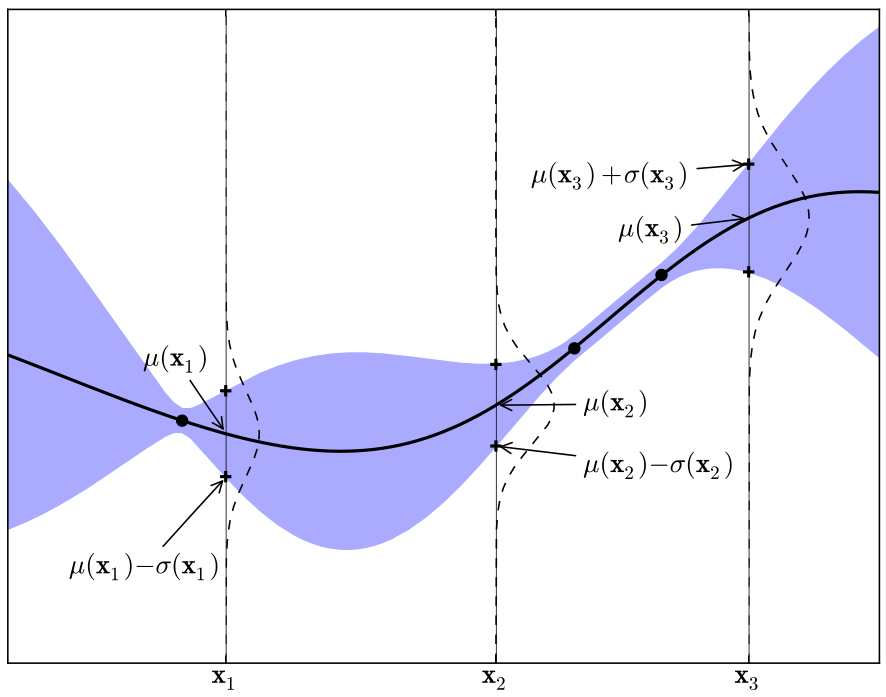
\includegraphics[scale=0.40]{figures/gp.png}
	\caption{Simple 1D Gaussian process with three observations. The solid black line is the GP surrogate mean prediction of the objective function given the data, and the shaded area shows the mean plus and minus the variance. The superimposed Gaussians correspond to the GP mean and standard deviation ($\mu(\cdot)$ and $\sigma(\cdot)$) of prediction at the points, $x_{1:3}$.}

	\label{fig:gp-example}
\end{figure}

%include regarding kernels
\subsection{Acquisition Functions}
Determines how we search for new points. For a Gaussian process prior, they are generally a function of three things: the mean of the hidden variable $f(x*)$, the standard deviation of $f(x*)$, and the best value seen so far during optimization, $y_{best}$.\\
Some acquisition functions are,
\begin{itemize}
	\item Probability of improvement
	\item Expected improvement
	\item Upper confidence bound
\end{itemize}

\section{Safe Bayesian Optimization}
\label{sec:safebo}
In safe Bayesian optimization instead of optimizing the unknown objective function $f(x)$ globally, it finds the maximizer within the safe set that is defined by safety constraints which not known to agent. 
So, this safe set is not known initially, but estimated after each safety constraints evaluation. So it is a technique, focused on solving the problem
$$ \max_{x_t\in\mathcal{X}}\text{ such that }g(x_t)\geq 0, \forall t\text{ with probability }\geq 1-\delta $$
\begin{figure}[h]
	\centering
	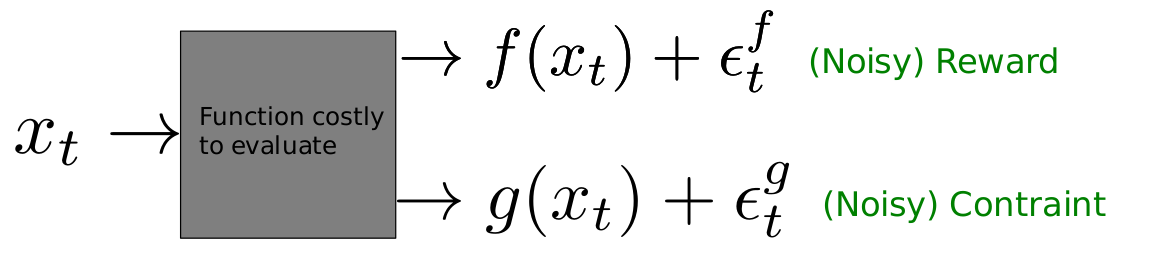
\includegraphics[scale=0.30]{figures/safebo.png}
	\caption{Safe Bayesian optimization illustration}
	\label{fig:safebo}
\end{figure}
\\
The formal problem setting of the safe Bayesian optimization can be explained by figure \ref{fig:safebo} (only one safety constrain is considered, could be multiple).
So at time $t$ agent select a action $x_t$ from the estimated safe set (every $x$ in the estimated safe set should satisfy the safety constrain with high probability.) and interact with the environment and observe the noisy observations $y_t$ and $z_t$ of the objective function $f(\cdot)$ and safety function $g(\cdot)$ at $x_t$ respectively. And add $(x_t , y_t , z_t )$ to the buffer or train set from which it update the Bayesian belief about the unknown objective and safety function.

\section{GP based Safe Exploration Algorithms}
A GP is well suited for safety-critical problem settings in which the unknown safety functions are modelled using GP, and the uncertainty of these functions are given by the confidence interval (i.e. variance) of their respective GPs. 
The confidence interval are used to take an action which is safe with high probability.
In the following section we will explain the SAFEOPT (safe exploration in Bandit or stateless setting).
\subsection{SafeOpt}
To guarantee safety in bandit setting problems Sui et al.\cite{sui15} proposed \texttt{SafeOpt} algorithm. The objective is to optimize a unknown function f (x) subject to safety constraint.
For that they have used safe Bayesian optimization framework (see section \ref{sec:safebo}). 
In their setting they considered the safety as, for chosen action/parameter $x_t$ at time $t$ the function value $f(x_t)$ should greater than a safety threshold $h$. 
Thus the authors approach the problem of estimating the maximum of the unknown function $f(x)$ by estimating $f(x)$ using Gaussian process (GP) regression. 
In GP regression, the unknown function is assumed to be modelled by a sample function from a GP prior \cite{RasmussenW06}. 
The GP prior is completely characterized by its mean function $\mu(x)$ (without loss of generality $\mu(x) = 0$) and covariance function $k(x, x^\prime )$ where $x, x^\prime \in \mathcal{X}$ . 
At every time $t$, the Safe-Opt policy chooses a point $x_t$ and receives an observation $y_t = f (x_t) + n_t$ where $n_t$ is an independent sample from Gaussian noise with mean 0 and variance $\sigma^2$. 
Based on $y_t$ a posterior distribution for the unknown function can be derived. 
This posterior distribution is again Gaussian and characterized completely by a mean function $\mu_t(x)$ and covariance function $k_t (x, x^\prime)$. 
In order to satisfy the safety constraints, Safe-Opt computes upper and lower confidence bounds on the function using this posterior. The upper $u_t(x)$ and lower $l_t(x)$ confidence bounds are defined as 
$$u_t(x)=\mu_t(x)+\beta_t\sigma_t(x),$$
$$l_t(x)=\mu_t(x)-\beta_t\sigma_t(x).$$
And it uses the confidence interval $Q_t(x) = [l_t(x), u_t(x)]$ to estimate a safe set $S_t\subset \mathcal{X}$, from which agent select a next query point $x_{t+1}$ for which the function value $f(x_{t+1})$ is greater than safety threshold with high probability. 
Safe Set $S_t$ is defined as:
$$ S_t \gets \cup_{x\in S_{t-1}}\{ x^\prime \in \mathcal{X} | l_t(x) - Ld(x,x^\prime) \geq h \} $$
where $L$ is lipschitz constant. 
SafeOpt assume at $t = 0$ it is provided with a initial safe seed $S_0$. 
Since the safe seed may not achieve the maxima of $f(x)$ it need to explore safely.
Safe-Opt maintains a set $G_t \subseteq S_t$ of candidate decisions that, upon potentially repeated selection, have a chance to expand $S_t$. The set $G_t$ is defined as
$$ G_t = \{x \in S_t | \psi_t(x) > 0 \} $$
where
$$ \psi_t(x) = |\{ x^\prime \in \mathcal{X} \backslash S_t | u_t(x) - Ld(x,x^\prime) \geq h \}| $$
In order to find the maxima SafeOpt maintain a another set $M_t \subseteq S_t$ of decisions that are potential maximizers of $f$.
$$ M_t = \{ x \in S_t |u_t(x) \geq \max_{x^\prime \in S_t} l_t(x^\prime) \} $$
Safe-Opt policy then chooses points $x_t$ according to $$ x_t = \argmax_{x\in G_t \cup M_t}w_t(x) $$
where $w_t(x)=u_t(x)-l_t(x)$.\\
The pseudo code for SafeOpt algorithm is given below. For high level description of SafeOpt please refer the Sui et. al. paper \cite{sui15}.
\begin{algorithm}
	\caption{\texttt{SafeOpt}}
	\label{alg:safeopt}
	\KwIn{Function domain $\mathcal{X}$ , GP prior $(\mu, k)$, signal variance parameter $\sigma_0$ , seed set $S_0$, safety threshold $h$, Lipschitz constant $L$.}
	$C_0(x) \gets [h, \infty), \forall x \in S_0$\\
	$C_0(x) \gets \mathbb{R}, \forall x \in \mathcal{X} - S_0$\\
	$Q_0(x) \gets \mathbb{R}, \forall x \in \mathcal{X}$\\
	\For{$t=1,\dots$}
	{
		$C_t(x) \gets C_{t-1}(x) \cap Q_{t-1}(x)$\\
		$S_t \gets \cup_{x\in S_{t-1}}\{ x^\prime \in \mathcal{X} | l_t(x) - Ld(x,x^\prime) \geq h \}$\\
		$G_t = \{x \in S_t | \psi_t(x) > 0 \}$\\
		$M_t = \{ x \in S_t |u_t(x) \geq \max_{x^\prime \in S_t} l_t(x^\prime) \}$\\
		$x_t = \argmax_{x\in G_t \cup M_t}w_t(x)$\\
		$y_t = f(x_t)+n_t$\\
		Compute $Q_t(x), \forall x \in S_t$\\
		if $\max_{ x\in G_t \cup M_t}w_t(x) \leq \epsilon$ then Break
	}
\end{algorithm}

\section{Parallel Bayesian Optimization}
Some ML models such as non-negative matrix factorization (NMF) have relatively few hyperparameters. 
However, emerging deep learning (DL) algorithms often consist of significantly more tunable parameters. 
As the number of model hyperparameters increases, their optimization becomes significantly more challenging as we face a combinatorial increase in potential model configurations. 
Similarly, there is an increased chance that our models' hyperparameters interact in complex ways. 
Modeling these interactions in high-dimensional search spaces quickly becomes challenging and can often defy our intuition. 
Even experts find it difficult to manually configure hyperparameters.

So, parallel optimization leverages high performance computing (HPC) resources to better understand unknown, potentially non-convex hyperparameter search spaces.

\subsection{Hyperspace}
\texttt{HyperSpace}\cite{YoungHRK18} approaches parallelism by concurrently running many Gaussian processes over our large hyperparameter search space. 
This is done by partitioning the hyperparameter search space, allowing us to model many regions of potential algorithm configurations. 
We emphasize the partitioning the search space since we are interested in how the changes of this optimization space affects our learner’s performance. 
This differs from the parallel approach presented in \cite{SnoekLA12}, where the authors parallelize a single Gaussian process. 
By running many GPs in parallel, we are able to compare our models' performance over various areas in the large hyperparameter search space as each GP grants a unique perspective over the
space. 
More critically, partitioning the search space means that a more detailed search is performed as many more models are explored across a diverse set of search spaces.

This addresses concerns of exponential scaling acknowledged in early papers on Bayesian optimization theory \cite{pmlr-v9-grunewalder10a} \cite{Srinivas.2012}, which showed that as number of search dimensions increase, Bayesian optimization requires many more queries of the objective function in order to bound our uncertainty about the optimization process, thus increasing the odds of finding near optimal values.

\subsubsection{Creating HyperSpaces}
The hyperparameter search space is divided as follows.
\begin{itemize}
	\item For each hyperparameter, we define a lower and an upper bound.
	\item We then divide each hyperparameter bound into two near equally sized subspaces with a degree of overlap, $ \phi \in [0,1] $.
	\item When $\phi=0$, there is no overlap between the subspaces.
	\item When $\phi=1$, there is perfect overlap and two copies of the original space are created.
	\item After dividing the original search space, we then create all possible combinations of these subintervals, what we call \textit{hyperspaces}.
\end{itemize}
A total of $2^H-S$ subspaces are created where $H$ is the number of hyperparameters whose interval bounds exceed some minimal length, $\alpha$, and $S$ is the number of hyperparameters whose interval bounds length is less than $\alpha$.
Each of these hyperspaces is subsequently distributed across an HPC(High Performance Computing) system.
At each node, we then run the Bayesian optimization loop for some predetermined $m$ iterations in parallel.\\

\begin{algorithm}[H] 
	\caption{\texttt{HyperSpace}}
	\KwIn{Hyperparameter intervals, minimal subinterval length $\alpha$, overlap $\phi$.}
	\KwOut{Optimization results over $2^N$ hyperspaces}
	\ForEach{hyperparameter interval}
	{
		\eIf{interval length $\geq \alpha$}
		{
			divide interval into two nearly equal subintervals with overlap $\phi$;
		}
		{
			do not split;
		}
	}
	combine all possible subintervals to form hyperspaces;\\
	\ForEach{hyperspace}
	{
		run Bayesian optimization;
	}
	\Return optimization results for each hyperspace
\end{algorithm}
\vspace{2em}
By leveraging HPC resources, HyperSpace is able to run $(2^H-S) * m$ iterations of Bayesian optimization in the time that it takes traditional SMBO algorithms to run $m$ iterations.

Figure \ref{fig:hspex} shows partitioning two hyperparameters with HyperSpace. Two hyperparameters, both integer valued, are each represented as a vector of eight elements. 
Each hyperparameter is divided into two equal subintervals, each consisting of four elements. 
Using $\phi = 0.25$, a single element from the lower and upper subintervals are appended to each subinterval respectively, making each subinterval of size five. The lower subinterval's maximum is now the minimum of the upper subinterval, and vice versa. 
Finally, all possible hyperparameter subintervals are combined to create the distributed search
spaces of HyperSpace.
\begin{figure}[h]
	\centering
	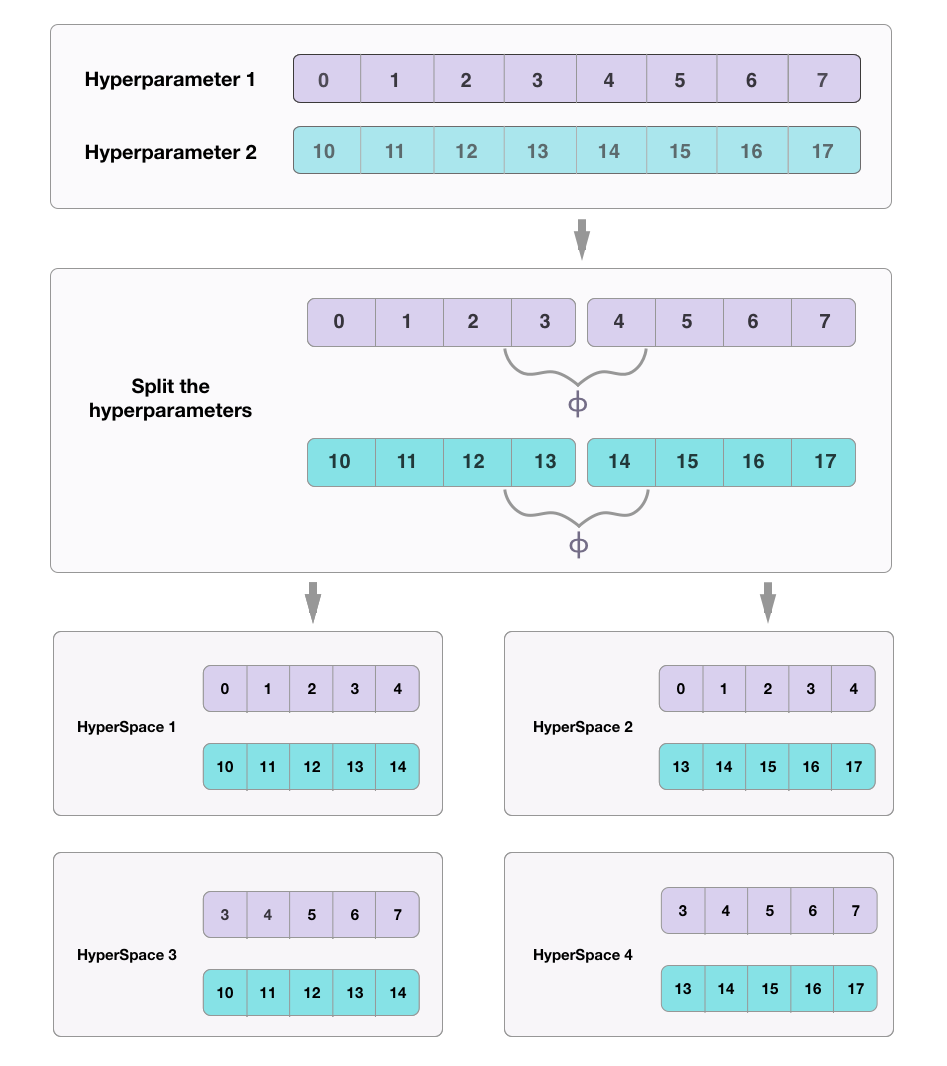
\includegraphics[scale=0.43]{figures/hyperspace-example.png}
	\caption{Partitioning two hyperparameters with HyperSpace}
	\label{fig:hspex}
\end{figure}
